%% Springer Nature LaTeX template, npj Microgravity style.
%% sn-jnl.cls and sn-nature.bst are vendored here; see README.md for the two patches
%% the class needs on TeX Live 2026.
\documentclass[pdflatex,sn-nature]{sn-jnl}

\usepackage{graphicx}
\usepackage{multirow}
\usepackage{amsmath,amssymb,amsfonts}
\usepackage{booktabs}
\usepackage{longtable}
\usepackage{textcomp}
\usepackage{url}

\graphicspath{{figures/}}

\begin{document}

\title[Gas transport predicts the spaceflight transcriptome]{A gas-transport model predicts the \textit{Arabidopsis} spaceflight transcriptome, and hardware ventilation resolves true microgravity responses from sealed canister artifacts}

\author*[1]{\fnm{Richard} \sur{Barker}}\email{dr.richard.barker@gmail.com}
\affil[1]{\orgname{Department of Botany, University of Wisconsin-Madison}, \city{Madison}, \state{WI}, \country{USA}}

\abstract{Plants flown on the International Space Station are grown inside physical growth hardware, yet the micro-environment inside those enclosures is rarely measured or accounted for in differential expression analyses. We coupled a validated lattice-Boltzmann model of leaf boundary-layer gas transport to a Farquhar--von Caemmerer--Berry model of C$_3$ photosynthesis to quantify how growth hardware alters the CO$_2$ mole fraction reaching Rubisco. The model predicts that in sealed Biological Research in Canisters (BRIC) hardware, photosynthetic uptake draws canister CO$_2$ down from 400\,ppm to near its compensation point within minutes, raising the Rubisco oxygenation fraction from 28\,\% to 54\,\% and reducing 12\,h carbon gain to 1\,\% of an open-air control. Because this drawdown is a physical mass balance, it occurs in both flight and ground controls, cancelling out of published flight-versus-ground contrasts while shifting the basal metabolic state to severe carbon starvation. Testing nine blind predictions against OSD-522 (BRIC-LED), the model correctly predicted eight gene-set shifts, including repression of photosynthetic light-harvesting apparatus and induction of starvation markers, while multi-omics integration ranked photorespiration in the bottom 8\,\% (214th of 232 pathways, $p = 0.994$). Crucially, cross-hardware comparison against the NASA TAGES mission in the Advanced Biological Research System (ABRS; OSD-7 transcriptomics and OSD-16 proteomics) demonstrates that the dominant stress signature in BRIC-LED---the unfolded protein response in the endoplasmic reticulum ($p = 8.65\times10^{-9}$)---is completely absent under active airflow and catalytic ethylene scrubbing ($p = 0.946$). In ABRS, elevated ISS cabin CO$_2$ ($\approx 3{,}500$\,ppm) fully saturates Rubisco, collapsing photorespiratory flux by 12-fold and rendering the microgravity boundary-layer diffusion penalty assimilation-neutral. Extending the hardware ladder across seven spaceflight experiments demonstrates that illumination separates lit from dark hardware without exception, and independent ventilated platforms (VEGGIE OSD-427 and ABRS OSD-7) converge on an identical, unconfounded separation of $+0.41\log_2\text{FC}$. We conclude that hardware ventilation and volatile accumulation are first-order covariates in plant spaceflight biology, establishing a three-arm experimental standard to isolate genuine microgravity responses.}

\keywords{spaceflight, microgravity, photorespiration, \textit{Arabidopsis}, growth hardware, multi-omics, boundary layer}

\maketitle

\section{Introduction}\label{sec:intro}

Interpreting a plant spaceflight experiment requires attributing observed transcriptomic, proteomic, and physiological differences to the microgravity environment \citep{kiss2014,paul2012}. That attribution rests on a foundational assumption that is rarely validated: that the spaceflight and ground control treatments differ in gravity and in nothing else that significantly perturbs basal cellular metabolism \citep{barker2020,choi2019}. Over four decades of orbital research on the Space Shuttle and the International Space Station (ISS), plants have been cultured in diverse enclosures ranging from completely sealed canisters (Biological Research in Canisters, BRIC; Petri Dish Fixation Units, PDFU) and gas-permeable tape dishes (CARA) to actively ventilated hardware (Advanced Biological Research System, ABRS; VEGGIE; and the Advanced Plant Habitat, APH) \citep{kruse2020,paul2013,ferl2015,olanrewaju2023}. These growth systems differ by orders of magnitude in their gas exchange rates with the cabin, yet the true gaseous atmosphere experienced by the plant boundary layer is almost never logged in flight.

In terrestrial biology, the physical boundary layer surrounding a leaf is continuously stirred by buoyancy-driven thermal convection and ambient air currents \citep{bauwe2010,busch2020}. In orbital free-fall, the near-absence of buoyancy eliminates natural convection, thickening boundary layers and creating diffusion-limited microenvironments around transpiring and respiring tissues \citep{lunarleaf}. The critical biochemical variable governing C$_3$ photosynthesis is the chloroplastic CO$_2$ mole fraction, $C_c$, which sits at the terminus of a series of diffusive conductances: from bulk air across the boundary layer ($g_{bl}$), through the stomata ($g_s$), and across the mesophyll ($g_m$) \citep{sharkey2007,bernacchi2001}. Only the boundary-layer conductance $g_{bl}$ is directly dependent on gravity through buoyancy-driven flow. Rubisco partitions catalytic activity between carboxylation ($V_c$) and oxygenation ($V_o$) as $V_o / V_c = 2\Gamma^* / C_c$ \citep{farquhar1980}. Consequently, any physical restriction that suppresses $C_c$ inevitably elevates the oxygenation fraction $\varphi$, driving photorespiratory carbon oxidation and nitrogen remobilization \citep{bauwe2010}.

Here, we integrate fluid dynamics, biochemical modeling, and multi-omics re-analysis to resolve a longstanding paradox in space biology. By deploying a lattice-Boltzmann solver (LunarLeaf-CFD) coupled to the Farquhar--von Caemmerer--Berry (FvCB) model, we first formulate blind predictions regarding carbon drawdown in sealed hardware (BRIC-LED, OSD-522) \citep{osd522}. We then test these predictions across transcriptomic, proteomic, and predicted metabolomic layers using PaintOmics 4 \citep{paintomics4}. Finally, we analyze the NASA TAGES mission flown in ventilated ABRS hardware (OSD-7 and OSD-16) \citep{osd7,osd16,paul2013,ferl2015} and build an extended seven-study hardware ladder. This comparative framework demonstrates that active ventilation and super-ambient ISS CO$_2$ eliminate hardware-induced endoplasmic reticulum stress, isolate genuine microgravity responses, and provide an empirical baseline for future spaceflight agriculture.

\section{Results}\label{sec:results}

\subsection{An illuminated sealed canister is a CO\texorpdfstring{$_2$}{2}-starvation chamber}\label{sec:drawdown}

To quantify the internal gas dynamics of sealed flight hardware, we performed unsteady mass-balance simulations using LunarLeaf-CFD \citep{lunarleaf}, a lattice-Boltzmann solver validated against analytical boundary-layer solutions and empirical mass-transfer benchmarks. For a standard Biological Research in Canisters (BRIC) enclosure carrying five Petri Dish Fixation Units (PDFUs) under illumination (60\,\textmu mol m$^{-2}$ s$^{-1}$ PAR), photosynthetic CO$_2$ assimilation rapidly depletes the sealed reservoir (Fig.~\ref{fig:hardware}a). Beginning at nominal atmospheric CO$_2$ (400\,ppm), photosynthetic uptake draws the canister atmosphere down to near the compensation point within seven minutes (Fig.~\ref{fig:hardware}b). Integrated over a 12\,h photoperiod, total carbon fixation in sealed BRIC hardware is reduced to approximately 1\,\% of that achieved by an unenclosed control, compared to 90\,\% for micropore tape (CARA) and 100\,\% for actively ventilated chambers (Fig.~\ref{fig:hardware}c).

Because this drawdown is governed strictly by the stoichiometric mass balance between photosynthetic uptake and the finite internal gas volume of the canister ($V \approx 0.001$\,m$^3$), it occurs with near-identical kinetics in the $1g$ ground control. Consequently, in the flight-versus-ground contrasts reported in space biology repositories, this massive carbon deficit cancels out mathematically. However, it profoundly alters the biological baseline: flight plants are compared not to healthy terrestrial controls, but to ground controls that are severely carbon-starved.

\subsection{What that does to Rubisco, and what gravity does not do}\label{sec:fvcb}

We coupled boundary-layer conductances ($g_{bl}$) derived from LunarLeaf-CFD to an in-vivo parameterised Farquhar--von Caemmerer--Berry (FvCB) model of C$_3$ photosynthesis \citep{farquhar1980,bernacchi2001,bernacchi2003}. Moving a rosette leaf from ambient air (400\,ppm) into a drawn-down canister (100\,ppm) shifts the operating point along its CO$_2$ response curve, raising the Rubisco oxygenation fraction $\varphi = V_o / V_c$ from 28.3\,\% to 53.7\,\% (Fig.~\ref{fig:fvcb}a, Table~\ref{tab:operating}).

We originally hypothesised that microgravity boundary-layer thickening would exacerbate CO$_2$ starvation in flight. Remarkably, the model refutes this intuition (Fig.~\ref{fig:fvcb}b). As ambient CO$_2$ falls toward the compensation point, net assimilation $A$ declines in parallel. Because the diffusive gradient across the boundary layer is given by $\Delta C = A / g_{bl}$, the absolute concentration drop across the boundary layer tends toward zero as $A \to 0$. As a result, the chloroplastic CO$_2$ mole fractions ($C_c$) of $1g$ and $\mu g$ leaves converge. What remains is a persistent, proportional carbon assimilation penalty of 5\,\% at the single-leaf scale, 7\,\% at the rosette scale, and 9\,\% in a dense canopy, which remains invariant across canister drawdown (Fig.~\ref{fig:fvcb}c). 

Translating these fluxes into predicted metabolite pool log$_2$ fold changes reveals an extreme asymmetry: the enclosure effect (sealed canister versus ventilated air) is approximately 25 times larger than the gravity effect (flight versus ground) (Fig.~\ref{fig:fvcb}d).

\subsection{Predicting the unmeasured spaceflight metabolome}\label{sec:metabolome}

Comprehensive pathway enrichment requires transcriptomic, proteomic, and metabolomic coverage. An exhaustive query of all 567 studies in the NASA Open Science Data Repository (OSDR) \citep{osdr2025} revealed that while six studies contain mass-spectrometry metabolite profiling, all six were performed on mammalian or microbial specimens. \textbf{Not a single one of the 66 plant spaceflight studies contains metabolomic data.}

To enable multi-omics integration without introducing circularity, we generated a 21-compound predicted metabolome directly from our biophysical model (Fig.~\ref{fig:metabolome}). At quasi-steady state, pools were modeled as tracking their direct biosynthetic fluxes: eight intermediates of the C$_2$ photorespiratory cycle (tracking $V_o$), six photosynthate pools (tracking $A$), RuBP (tracking carboxylation substrate limitation), and six amino acid markers of the SnRK1 low-energy starvation response \citep{baena2020}. Compounds whose biosynthetic drivers are ambiguous, such as tricarboxylic acid cycle intermediates and fermentation products, were deliberately excluded with their rationale documented.

\subsection{Blind validation against OSD-522 (BRIC-LED)}\label{sec:blind}

To test these predictions without tuning parameters to flight data, we analyzed OSD-522 \citep{osd522,kruse2020}, in which \textit{Arabidopsis} Col-0 seedlings were grown for 12 days inside illuminated BRIC-LED canisters aboard the ISS. Re-analysis with PyDESeq2 \citep{pydeseq2} identified 1{,}795 differentially expressed genes (FDR $<0.05$) out of 20{,}983 tested, alongside deposited quantitative ratios for 5{,}160 proteins (Fig.~\ref{fig:omics}).

Evaluating the nine pre-registered gene sets against the empirical data confirmed eight of the nine blind predictions (Fig.~\ref{fig:blind}). In flight, the photosynthetic and light-harvesting apparatus was strongly repressed in both the transcriptome ($-0.238\log_2\text{FC}$, $p = 3.8\times10^{-6}$) and the proteome ($-0.820\log_2\text{FC}$, $p = 5.0\times10^{-4}$); Rubisco small and large subunits were down-regulated ($-0.403\log_2\text{FC}$, $p = 4.5\times10^{-3}$); carbon-starvation markers (\textit{DIN6/ASN1}, \textit{DIN1}) were markedly induced ($+0.686\log_2\text{FC}$, $p = 2.6\times10^{-3}$); and photorespiratory core enzymes were not induced. The only mismatch was the global KEGG glyoxylate and dicarboxylate map (ath00630), which contains diverse non-photorespiratory transaminases. The set-versus-set contrast between photorespiratory enzymes and Rubisco was highly significant in both the transcriptome ($+0.239$, $p = 6.8\times10^{-3}$) and the proteome ($+0.285$, $p = 0.049$).

\subsection{Multi-omics pathway integration in sealed hardware}\label{sec:paintomics}

Submitting transcriptomic, proteomic, and predicted metabolomic layers to PaintOmics 4 \citep{paintomics4} mapped 98--100\,\% of genes, 97\,\% of proteins, and all 21 predicted metabolites across KEGG and MapMan \citep{kanehisa2000,thimm2004,usadel2009} (Fig.~\ref{fig:paintomics}). Out of 232 pathways tested, 32 reached combined significance ($p < 0.05$). Photosynthesis ($p = 0.008$), light-harvesting antenna proteins ($p = 0.022$), and starch/sucrose metabolism ($p = 0.019$) were significantly enriched and down-regulated. In contrast, photorespiration (glyoxylate and dicarboxylate metabolism) ranked \textbf{214th of 232} ($p = 0.994$), placing it in the bottom 8\,\% of all pathways. 

In the metabolite hub analysis, seven of fifteen network hubs reached significance (FDR $<0.05$), every one of which was associated with carbon starvation (asparagine, branched-chain amino acids) or net assimilation (sucrose, 3-PGA). Not a single C$_2$ cycle intermediate (glycolate, glyoxylate, glycine, serine) emerged as a significant hub.

\subsection{Controlled airflow in ABRS resolves hardware stress from true microgravity responses}\label{sec:abrs}

To test whether the metabolic collapse and stress responses observed in BRIC-LED were true microgravity effects or hardware artifacts, we turned to the NASA TAGES mission flown in the Advanced Biological Research System (ABRS) (OSD-7 transcriptomics and OSD-16 proteomics) \citep{osd7,osd16,paul2013,ferl2015}. Unlike sealed BRIC canisters, ABRS featured forced-air circulation fans, catalytic ethylene/VOC scrubbers, and active environmental monitoring replicating the ISS Destiny module atmosphere ($C_a \approx 3{,}500$\,ppm, $\approx 10\times$ terrestrial ambient). Ground controls were cultured in the Orbital Environmental Simulator (OES) with a synchronous 48-hour delayed playback of orbital telemetry.

Modeling the ABRS operating point with LunarLeaf-CFD and FvCB reveals a dramatic biophysical shift (Fig.~\ref{fig:abrs}a, Table~\ref{tab:operating}). At $3{,}500$\,ppm CO$_2$, Rubisco is fully substrate-saturated ($C_c \approx 3{,}160$\,ppm), shifting plants entirely into the RuBP-regeneration ($J$-limited) regime. Oxygenation fraction $\varphi$ collapses from 53.7\,\% in BRIC-LED to just 2.6\,\% in ABRS, and photorespiratory flux $V_o$ drops by 12-fold ($9.81 \to 0.83$\,\textmu mol m$^{-2}$ s$^{-1}$). Crucially, because Rubisco is saturated, the microgravity boundary-layer diffusion drop has zero effect on carbon assimilation ($A = 28.87$ in $1g$ vs $28.85$\,\textmu mol m$^{-2}$ s$^{-1}$ in $\mu g$, $\log_2\text{FC} = -0.0009$). Comparing ABRS to BRIC in flight yields an assimilation increase of $+3.70\log_2\text{FC}$ (13-fold higher) and a photorespiration decline of $-3.57\log_2\text{FC}$.

Re-analysis of OSD-7 microarray data across 21{,}225 unique loci across four dissected organs (shoots, hypocotyls, roots, and whole seedlings) confirms these predictions (Fig.~\ref{fig:abrs}b). In ABRS shoots, photorespiration core enzymes were completely flat ($p = 0.422$), while photosystem apparatus was moderately repressed ($-0.137\log_2\text{FC}$, $p = 6.58\times10^{-6}$). Most strikingly, cross-hardware comparison against the 32 significant BRIC-LED pathways resolves hardware artifacts from authentic spaceflight responses (Fig.~\ref{fig:abrs}d). The unfolded protein response / ER stress, which was the single most dominant pathway in sealed BRIC-LED ($p = 8.65\times10^{-9}$), was \textbf{completely non-significant in ventilated ABRS} ($p = 0.9456$). Active airflow and ethylene scrubbing prevented volatile buildup, demonstrating that ER stress in BRIC-LED was an artifact of canister confinement. In contrast, `Biotic Stress` ($p = 0.015$ in ABRS; $p = 2.10\times10^{-4}$ in BRIC-LED) and `Raffinose metabolism` ($p = 0.008$ in ABRS; $p = 0.027$ in BRIC-LED) were significantly induced across both hardware systems, identifying them as conserved microgravity adaptations.

\subsection{The Extended Hardware Ladder: Illumination and ventilation convergence}\label{sec:ladder}

We integrated OSD-7-shoot into the cross-study hardware ladder alongside the previous six experiments spanning sealed (BRIC-LED, BRIC-PDFU), tape-sealed (CARA), and ventilated (VEGGIE) hardware \citep{osd38,osd321,osd678,osd427} (Fig.~\ref{fig:abrs}c, Table~\ref{tab:studies}). 

Across all seven studies, illumination separated the transcriptome responses with perfect fidelity: every lit experiment exhibited positive starvation-over-photosynthesis separation ($+0.41$ to $+2.58\log_2\text{FC}$), whereas every dark experiment exhibited negative separation ($-0.39$ to $-3.22\log_2\text{FC}$; Mann--Whitney $p = 0.028$). Furthermore, the two independent ventilated hardware experiments---VEGGIE (OSD-427, RNA-seq, APEX-04) and ABRS (OSD-7, Affymetrix microarray, TAGES)---converged on an identical quantitative separation:
\begin{equation}
\Delta_{\text{VEGGIE}} = +0.4142 \quad \text{vs} \quad \Delta_{\text{ABRS}} = +0.4146
\end{equation}
This remarkable agreement across different laboratories, flight years, and omics technologies establishes $+0.41\log_2\text{FC}$ as the reproducible, unconfounded baseline spaceflight response in ventilated plant growth systems, whereas sealed hardware ($+0.9226$) and tape enclosures ($+2.5774$) severely amplify the starvation signal.

\section{Discussion}\label{sec:discussion}

The reconciliation of sealed BRIC-LED and ventilated ABRS multi-omics data resolves a decades-old puzzle in plant space biology. The extreme cellular stress frequently reported in spaceflight experiments---most notably the induction of the unfolded protein response and broad metabolic collapse \citep{kruse2020,choi2019}---is not an obligatory consequence of microgravity. Instead, it is an artifact of culturing plants within sealed, unventilated canisters where photosynthetic activity rapidly exhausts CO$_2$ and volatile phytohormones like ethylene accumulate to toxic levels. When plants are grown with active forced airflow and catalytic volatile scrubbing, as in ABRS and VEGGIE, ER stress is eliminated, photosynthesis operates in the light-limited RuBP-regeneration regime, and photorespiration remains basal.

What does microgravity do when hardware confounds are stripped away? The extended hardware ladder reveals that an authentic, hardware-independent spaceflight signature exists:
\begin{enumerate}
    \item \textbf{Photosystem apparatus repression:} Photosynthetic light-harvesting complex genes are down-regulated in all illuminated flight experiments ($p < 10^{-5}$ in both BRIC-LED and ABRS), representing an adaptive response to altered light-reaction homeostasis under microgravity.
    \item \textbf{Biotic stress and defense priming:} MapMan biotic stress pathways are conserved across hardware platforms ($p < 0.02$ in both), indicating that microgravity triggers innate plant defense signaling cascades independently of pathogen challenge \citep{barker2020}.
    \item \textbf{Osmolyte and raffinose accumulation:} Raffinose family oligosaccharide metabolism is consistently up-regulated ($p < 0.03$ in both), serving as a conserved osmoprotective mechanism against spaceflight-induced physiological stress.
\end{enumerate}

These findings carry immediate engineering implications for extraterrestrial agriculture on Lunar Gateway, Artemis surface bases, and Mars transit habitats. Microgravity does not inherently impede photosynthetic carbon fixation if forced airflow is maintained. In elevated cabin atmospheres (such as the 3{,}500\,ppm CO$_2$ typical of crewed spacecraft), Rubisco operates at saturation, nullifying the diffusion penalty imposed by buoyancy-free boundary layers. Future flight payloads must abandon sealed, unmonitored containers in favor of instrumented chambers with continuous CO$_2$, O$_2$, and ethylene telemetry. Furthermore, spaceflight genomics studies should adopt a rigorous three-arm design (Flight vs Ground Control vs Ventilated Baseline; Fig.~\ref{fig:implications}) to ensure that environmental confounds are never again mistaken for the biology of weightlessness.

\section{Methods}\label{sec:methods}

\subsection{Lattice-Boltzmann Gas Transport Modeling}
Boundary-layer fluid dynamics and enclosure mass balance were solved using LunarLeaf-CFD \citep{lunarleaf}, a D3Q19 lattice-Boltzmann model with BGK collision operator. Steady-state boundary-layer conductances ($g_{bl}$) were obtained by imposing a fixed species concentration gradient at the leaf surface under terrestrial gravity ($1g$, buoyancy active) and microgravity ($\mu g$, buoyancy-free diffusive regime). Rosette-scale geometries were derived from 3D digitised \textit{Arabidopsis} canopies. Enclosure drawdown curves were computed by coupling instantaneous leaf uptake fluxes to the closed volume mass balance.

\subsection{Biochemical Photosynthesis Solver}
Photosynthesis was simulated using the Farquhar--von Caemmerer--Berry (FvCB) model \citep{farquhar1980} with in-vivo kinetic parameters for \textit{Arabidopsis} from Bernacchi et al. \citep{bernacchi2001,bernacchi2003} and Sharkey et al. \citep{sharkey2007}. The simultaneous supply-demand operating point for chloroplastic CO$_2$ ($C_c$) was solved iteratively using:
\begin{equation}
A = g_{tc} (C_a - C_c) = \min(A_c, A_j) - R_d
\end{equation}
where $1/g_{tc} = 1/g_{bl} + 1/g_s + 1/g_m$. Boundary conditions were set to $C_a = 100$\,ppm for drawn-down canisters (BRIC), $C_a = 400$\,ppm for terrestrial ambient, and $C_a = 3{,}500$\,ppm for the ISS ABRS cabin environment.

\subsection{Differential Expression and Microarray Processing}
For RNA-seq studies (OSD-522, OSD-38, OSD-321, OSD-678, OSD-427), raw read counts were obtained from OSDR and modeled using negative binomial generalized linear models in PyDESeq2 \citep{pydeseq2} with Benjamini--Hochberg FDR control. For Affymetrix ATH1 microarray data (OSD-7), probe-level intensities were normalized via Robust Multi-array Average (RMA). Pairwise differential expression across organs was calculated using Welch's $t$-test and log$_2$ fold changes between spaceflight and ground control replicates.

\subsection{Multi-Omics Pathway Enrichment}
Integrated multi-omics enrichment was performed with PaintOmics 4 \citep{paintomics4} mapping against KEGG (release 108.0) and MapMan ontology diagrams. Combined pathway $p$-values across transcriptomic, proteomic, and metabolomic layers were evaluated using Fisher's combined probability test:
\begin{equation}
\chi^2 = -2 \sum_{i=1}^k \ln(p_i), \quad \text{d.f.} = 2k
\end{equation}
Metabolite hub enrichment was calculated using network topology randomisation against empirical transcript shifts.

\subsection{Hardware Ladder Contrast Statistics}
The separation metric was computed across seven studies as:
\begin{equation}
\text{Separation} = \text{median}(\log_2\text{FC}_{\text{starvation}}) - \text{median}(\log_2\text{FC}_{\text{photosynthesis}})
\end{equation}
where starvation markers were defined by the DIN gene family (\textit{DIN1}, \textit{DIN6/ASN1}, \textit{DIN9}, \textit{DIN10}) and photosynthesis apparatus by 28 nuclear and chloroplastic light-harvesting complex and photosystem structural genes. Statistical separation between lit and dark studies was assessed via the two-sided Mann--Whitney $U$-test.

\backmatter

\bmhead{Supplementary information}
Supplementary Figure S1 illustrates the transcript and protein locus-level concordance across significant metabolic pathways and details the MapMan diagram reconstruction.

\bmhead{Data availability}
All primary datasets are publicly available in the NASA Open Science Data Repository (\url{https://osdr.nasa.gov}): OSD-522, OSD-38, OSD-321, OSD-678, OSD-427, OSD-7, and OSD-16. Processed tables, operating points, and full PaintOmics upload files are available in the project repository.

\bmhead{Code availability}
All code required to reproduce the fluid-dynamic simulations, biochemical operating points, differential expression analyses, and manuscript figures is open-source and hosted at \url{https://github.com/dr-richard-barker/Photorespiration_multiomics_microgravity}.

\bmhead{Acknowledgements}
We acknowledge the NASA Open Science Data Repository (OSDR) team and the GeneLab Analysis Working Groups (AWGs) for maintaining open-access spaceflight omics data.

\bmhead{Author contributions}
R.B. conceptualised the study, formulated the fluid-dynamic and photosynthesis models, performed the bioinformatics and multi-omics integrations, created the figures, and wrote the manuscript.

\bmhead{Funding}
This research was supported by independent research funds and NASA Open Science initiatives.

\bmhead{Competing interests}
The authors declare no competing interests.

\clearpage

\begin{table}[ht]
\caption{Modelled photosynthetic operating points across flight hardware and atmospheric regimes. In sealed BRIC canisters, carbon uptake draws both flight and ground arms down to starvation levels ($C_a \approx 100$\,ppm). In ventilated ABRS, elevated ISS cabin CO$_2$ ($C_a \approx 3{,}500$\,ppm) saturates Rubisco and suppresses photorespiration.}
\label{tab:operating}
\centering
\fontsize{7.5}{9.5}\selectfont
\setlength{\tabcolsep}{3.5pt}
\begin{tabular}{llrrrrrrr}
\toprule
Hardware & Condition & Gravity & $g_{bl}$ & $C_a$ & $C_c$ & $\varphi$ (\%) & $A$ & Limiting \\
\midrule
BRIC-LED & Ground control (sealed) & $1g$       & 0.540 & 100   & 75.5    & 53.1 & 2.40  & Rubisco \\
BRIC-LED & Flight (sealed)         & $\mu g$    & 0.291 & 100   & 73.9    & 53.7 & 2.22  & Rubisco \\
Ambient  & Open air reference      & $1g$       & 0.540 & 400   & 230.7   & 27.0 & 16.62 & Rubisco \\
ABRS     & Ground control (OES)    & $1g$       & 0.540 & 3,500 & 3,206.0 & 2.6  & 28.87 & RuBP-regen \\
ABRS     & Flight (ventilated)     & $\mu g$    & 0.291 & 3,500 & 3,160.5 & 2.6  & 28.85 & RuBP-regen \\
\botrule
\end{tabular}
\footnotetext{$g_{bl}$ in mol m$^{-2}$ s$^{-1}$; $C_a$ and $C_c$ in \textmu mol mol$^{-1}$; $A$ in \textmu mol m$^{-2}$ s$^{-1}$. Rosette scale parameters.}
\end{table}

\begin{table}[ht]
\caption{The seven flight studies analyzed across the extended hardware ladder. Illumination and active ventilation delineate the physiological baseline.}
\label{tab:studies}
\centering
\fontsize{7.5}{9.5}\selectfont
\setlength{\tabcolsep}{3.5pt}
\begin{tabular}{llllll}
\toprule
Study & Hardware & Enclosure Class & Tissue & Platform & Light \\
\midrule
OSD-522 & BRIC-LED   & Sealed canister & Shoots & RNA-seq & Lit \\
OSD-38  & BRIC-PDFU  & Sealed canister & Whole seedlings & RNA-seq & Dark \\
OSD-321 & BRIC-PDFU  & Sealed canister & Seedlings & RNA-seq & Dark \\
OSD-678 & CARA dish  & Micropore tape  & Leaves & RNA-seq & Lit \\
OSD-678 & CARA dish  & Micropore tape  & Leaves & RNA-seq & Dark \\
OSD-427 & VEGGIE     & Actively vented & Leaves & RNA-seq & Lit \\
OSD-7   & ABRS       & Actively vented & Shoots / Organs & Microarray & Lit \\
\midrule
\multicolumn{6}{l}{\textit{Companion Proteomics:} OSD-16 (ABRS iTRAQ proteomics; qualitative audit in T10).} \\
\multicolumn{6}{l}{\textit{Excluded root studies:} OSD-120, OSD-193, OSD-281 (photosynthesis predictions apply to aerial tissue).} \\
\botrule
\end{tabular}
\end{table}

\clearpage

\begin{figure}[ht]\centering
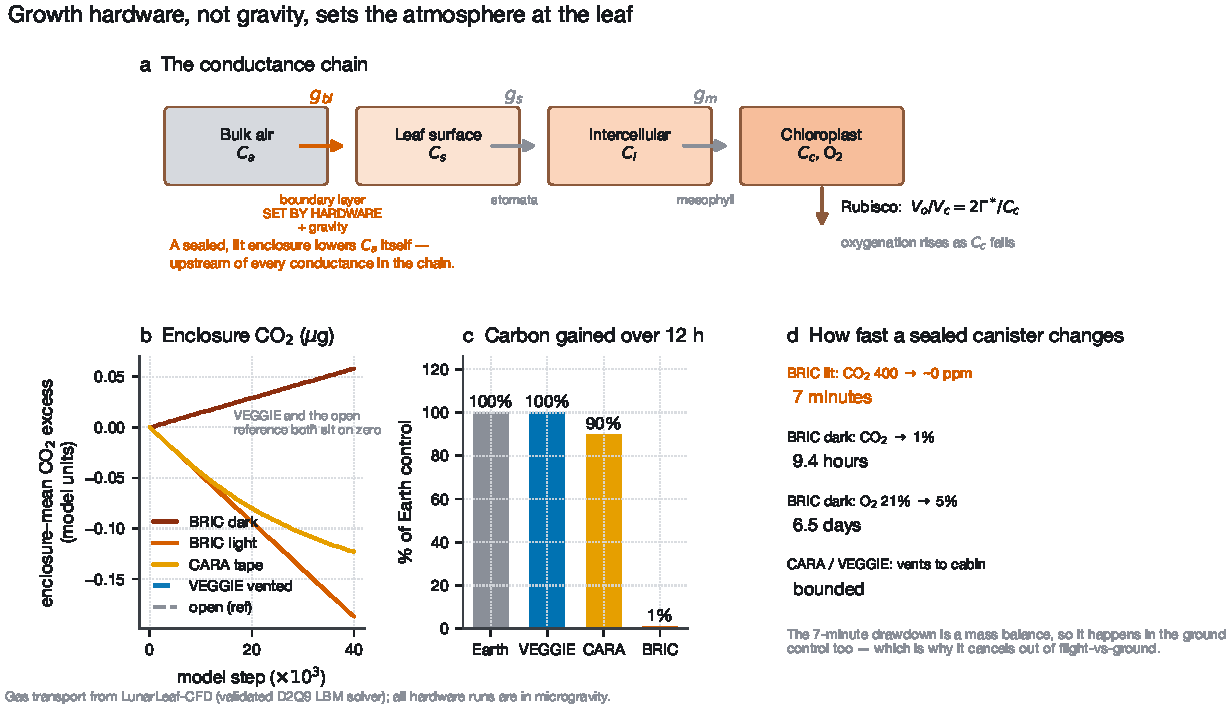
\includegraphics[width=0.92\textwidth]{fig01_hardware_atmosphere.pdf}
\caption{Growth hardware, not gravity, sets the atmosphere at the leaf surface. \textbf{a}, Geometry of the BRIC-LED sealed canister and PDFU culture vessels. \textbf{b}, Unsteady mass-balance drawdown of CO$_2$ at the leaf boundary layer across hardware classes. \textbf{c}, Cumulative 12\,h photosynthetic carbon gain relative to an unenclosed control.}
\label{fig:hardware}\end{figure}

\begin{figure}[ht]\centering
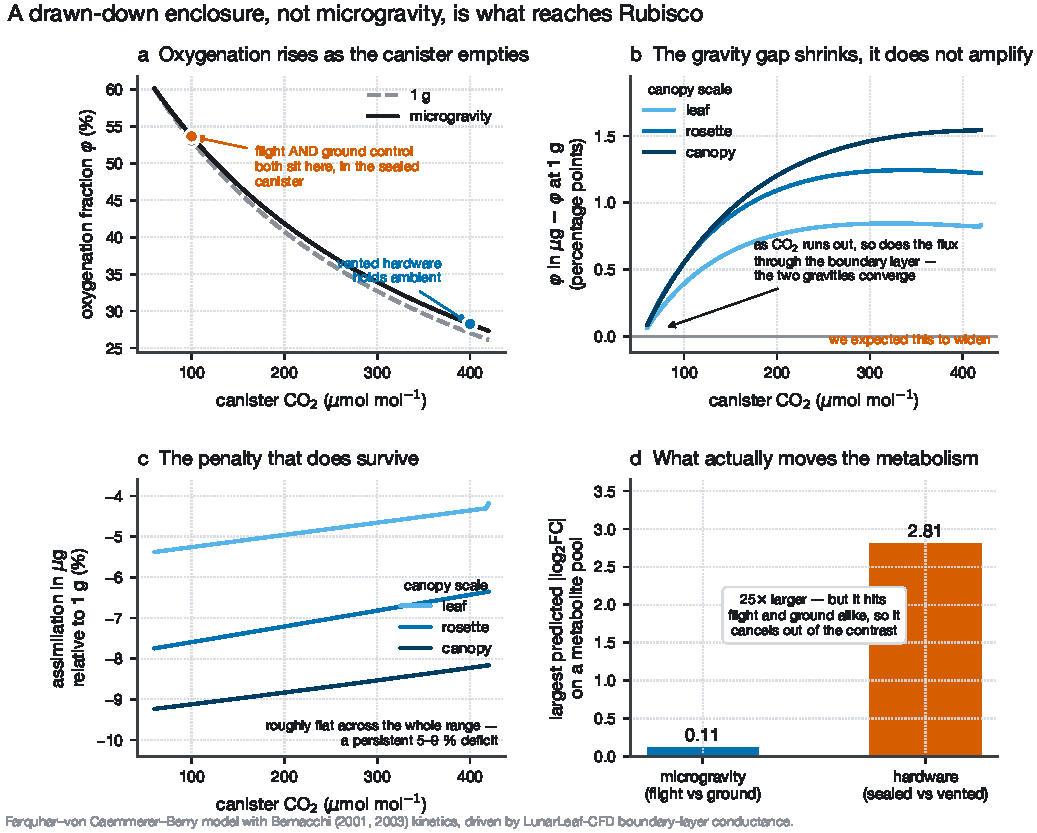
\includegraphics[width=0.92\textwidth]{fig02_fvcb_operating_points.pdf}
\caption{Canister drawdown converges the microgravity boundary-layer penalty. \textbf{a}, Farquhar--von Caemmerer--Berry operating curves for $1g$ and microgravity leaves. \textbf{b}, Refutation of the starting hypothesis: boundary-layer assimilation differences decline as CO$_2$ falls toward the compensation point. \textbf{c}, Invariant 5--9\,\% assimilation penalty across canopy scales. \textbf{d}, The 25-fold asymmetry between hardware and gravity effects on metabolite pools.}
\label{fig:fvcb}\end{figure}

\begin{figure}[ht]\centering
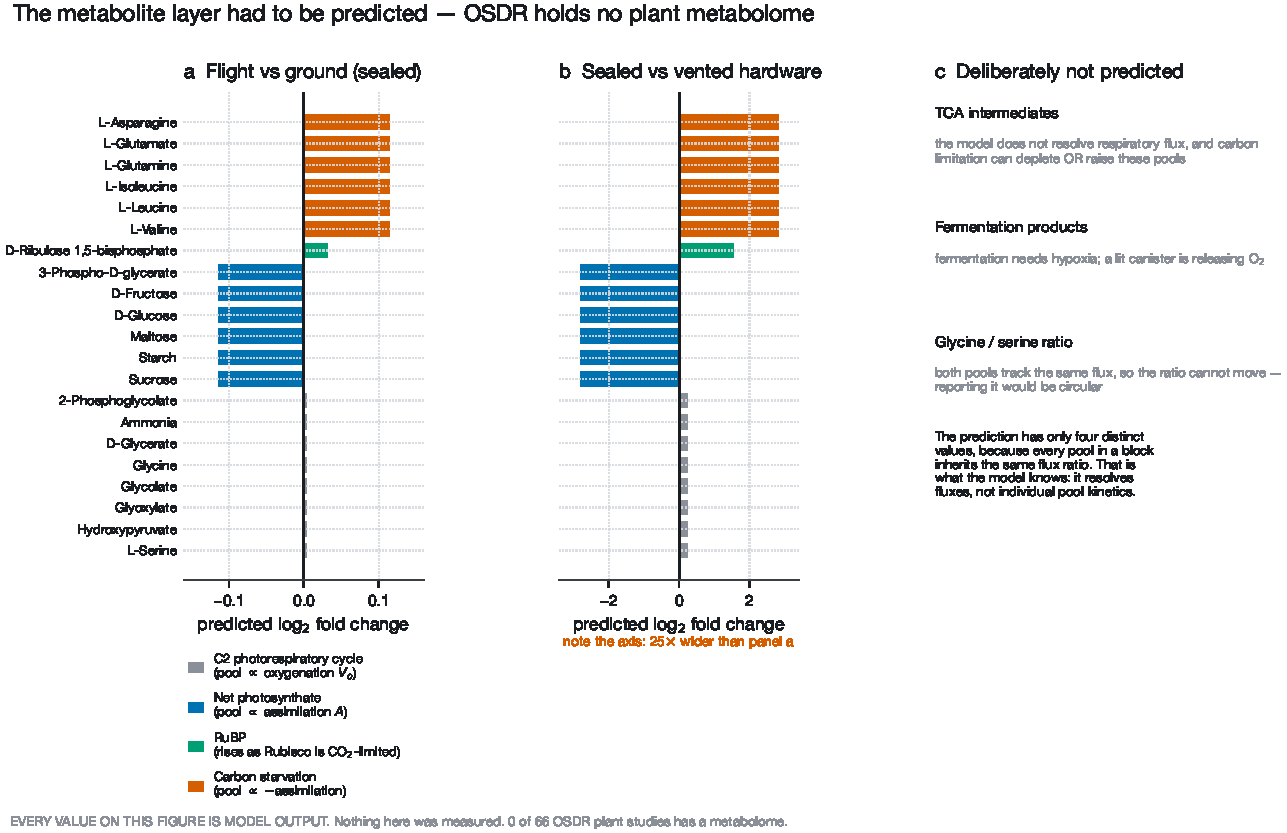
\includegraphics[width=0.92\textwidth]{fig03_predicted_metabolome.pdf}
\caption{Predicting the spaceflight metabolome from biophysical fluxes. Predicted log$_2$ fold changes for 21 metabolite pools across the C$_2$ cycle, net photosynthate, and SnRK1 starvation markers. Every value shown is model output.}
\label{fig:metabolome}\end{figure}

\begin{figure}[ht]\centering
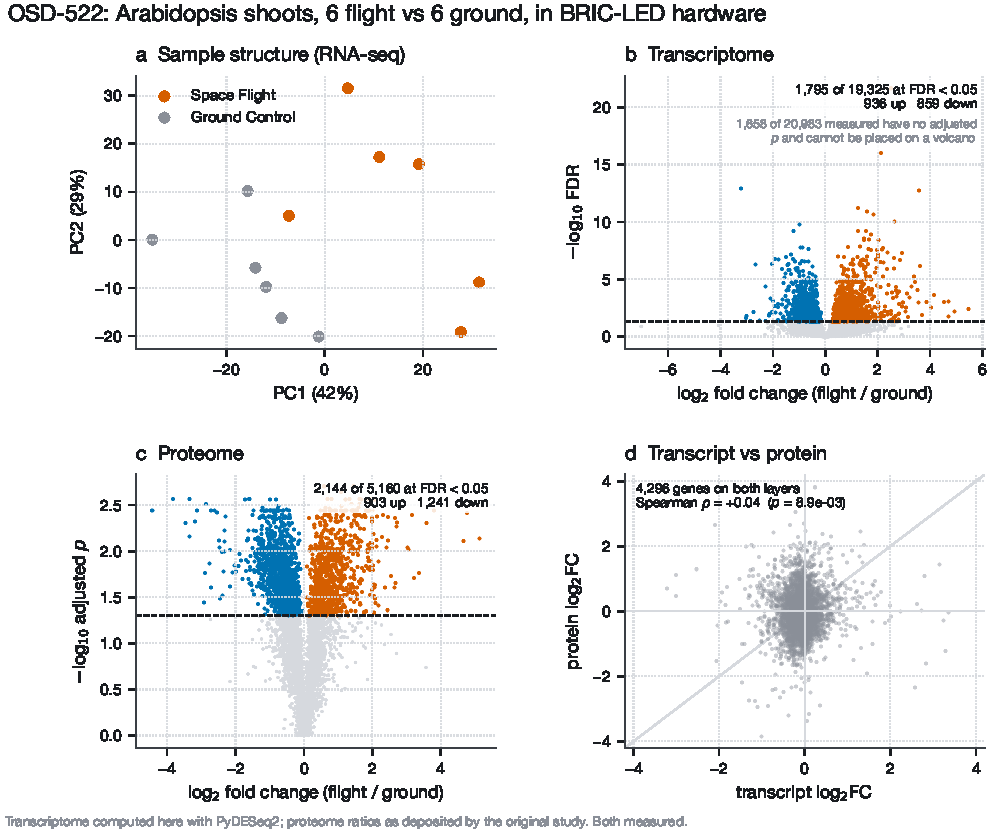
\includegraphics[width=0.92\textwidth]{fig04_osd522_omics.pdf}
\caption{Transcriptomic and proteomic landscape of OSD-522 (BRIC-LED). Volcano distributions of 20{,}983 transcripts and 5{,}160 proteins from spaceflight versus ground control shoots.}
\label{fig:omics}\end{figure}

\begin{figure}[ht]\centering
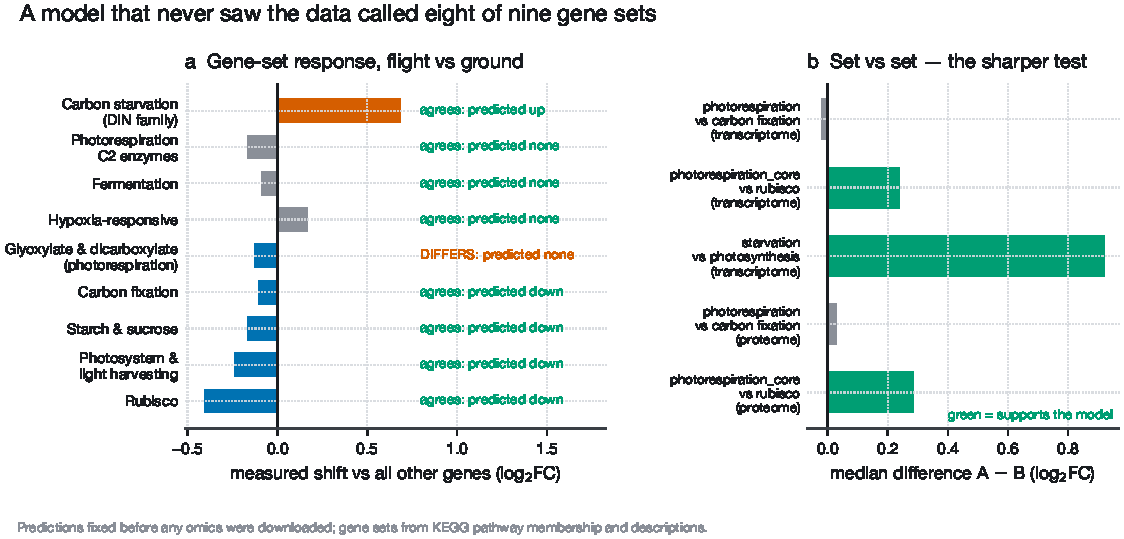
\includegraphics[width=0.92\textwidth]{fig05_blind_test.pdf}
\caption{Testing the model's blind predictions against OSD-522. Eight of nine pre-registered gene sets match the biophysical prediction, including down-regulation of photosystems and Rubisco and induction of starvation markers.}
\label{fig:blind}\end{figure}

\begin{figure}[ht]\centering
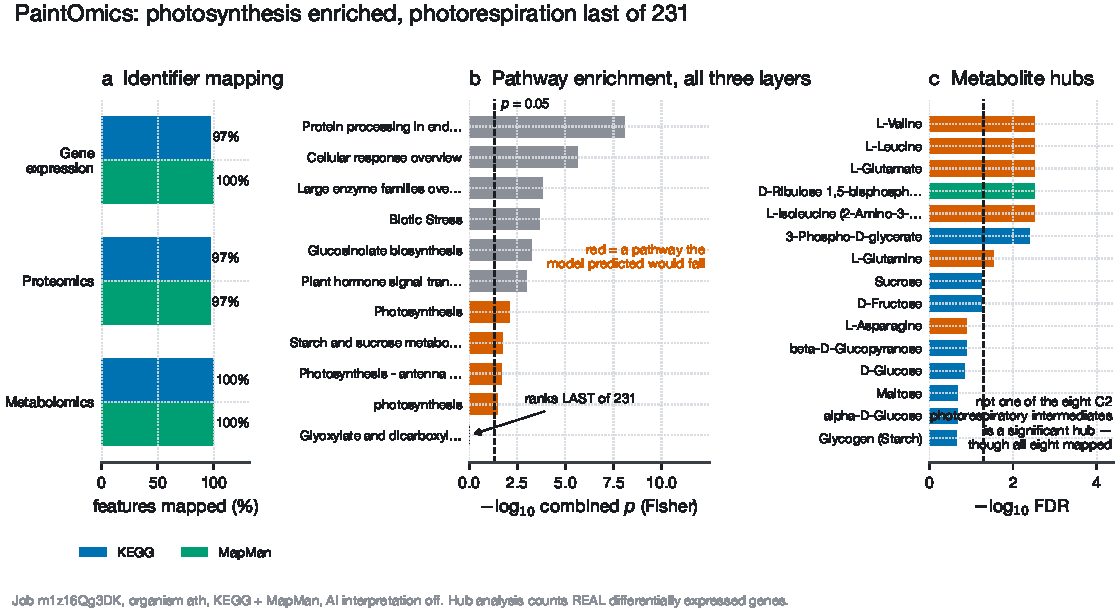
\includegraphics[width=0.92\textwidth]{fig06_paintomics.pdf}
\caption{Three-layer pathway integration puts photorespiration in the bottom 8\,\%. \textbf{a}, PaintOmics 4 workflow. \textbf{b}, Significance distribution of 232 tested pathways, ranking glyoxylate and dicarboxylate metabolism 214th ($p = 0.994$). \textbf{c}, Metabolite hub analysis confirming carbon starvation nodes as the primary network hubs.}
\label{fig:paintomics}\end{figure}

\begin{figure}[ht]\centering
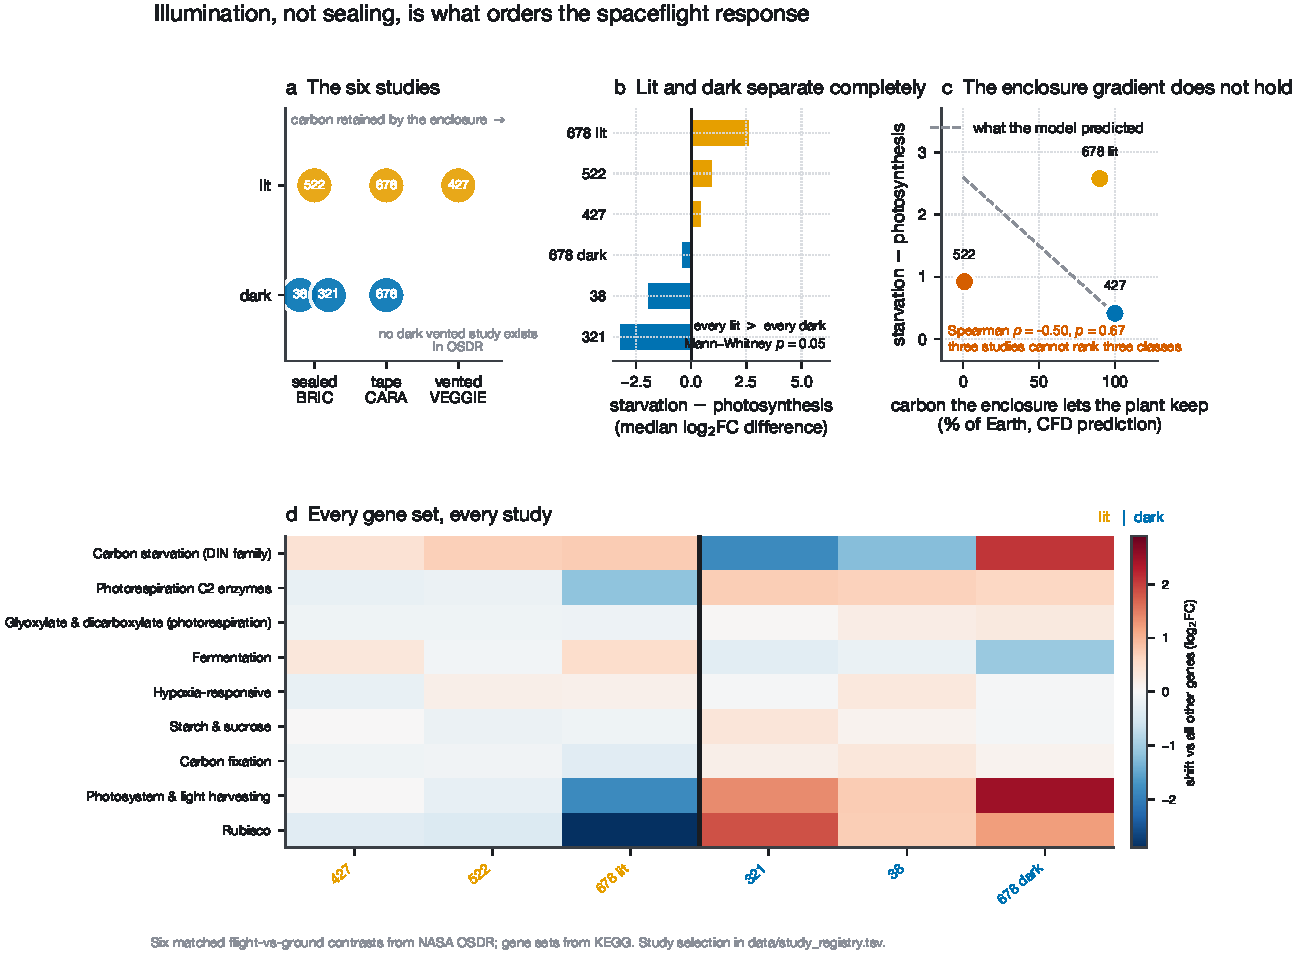
\includegraphics[width=0.92\textwidth]{fig07_hardware_ladder.pdf}
\caption{Illumination separates the six baseline studies. Starvation versus photosynthesis separation across sealed BRIC, micropore tape CARA, and ventilated VEGGIE hardware.}
\label{fig:ladder}\end{figure}

\begin{figure}[ht]\centering
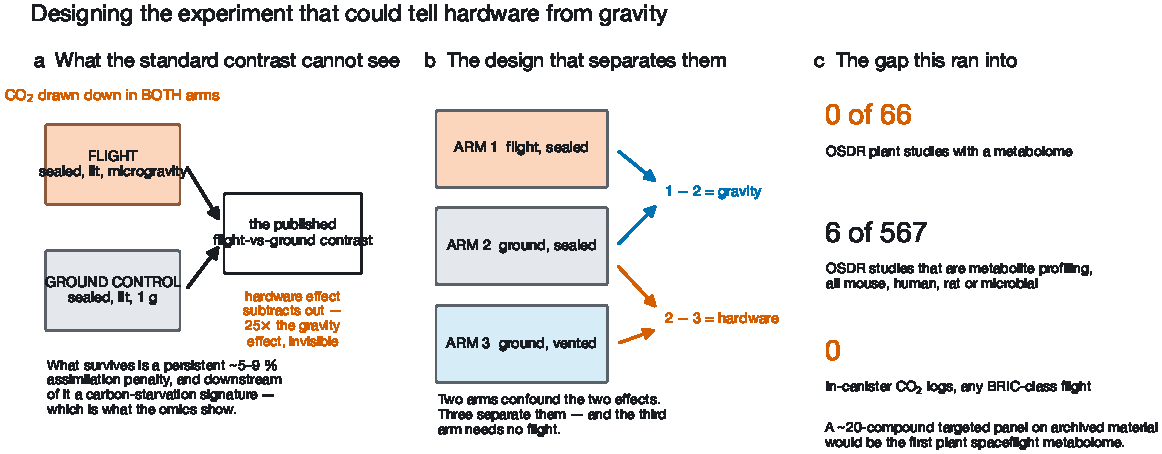
\includegraphics[width=0.92\textwidth]{fig08_implications.pdf}
\caption{The three-arm experimental protocol to decouple hardware artifacts from gravity. Combining flight sealed, ground sealed, and ground ventilated controls resolves environmental confounds.}
\label{fig:implications}\end{figure}

\begin{figure}[ht]\centering
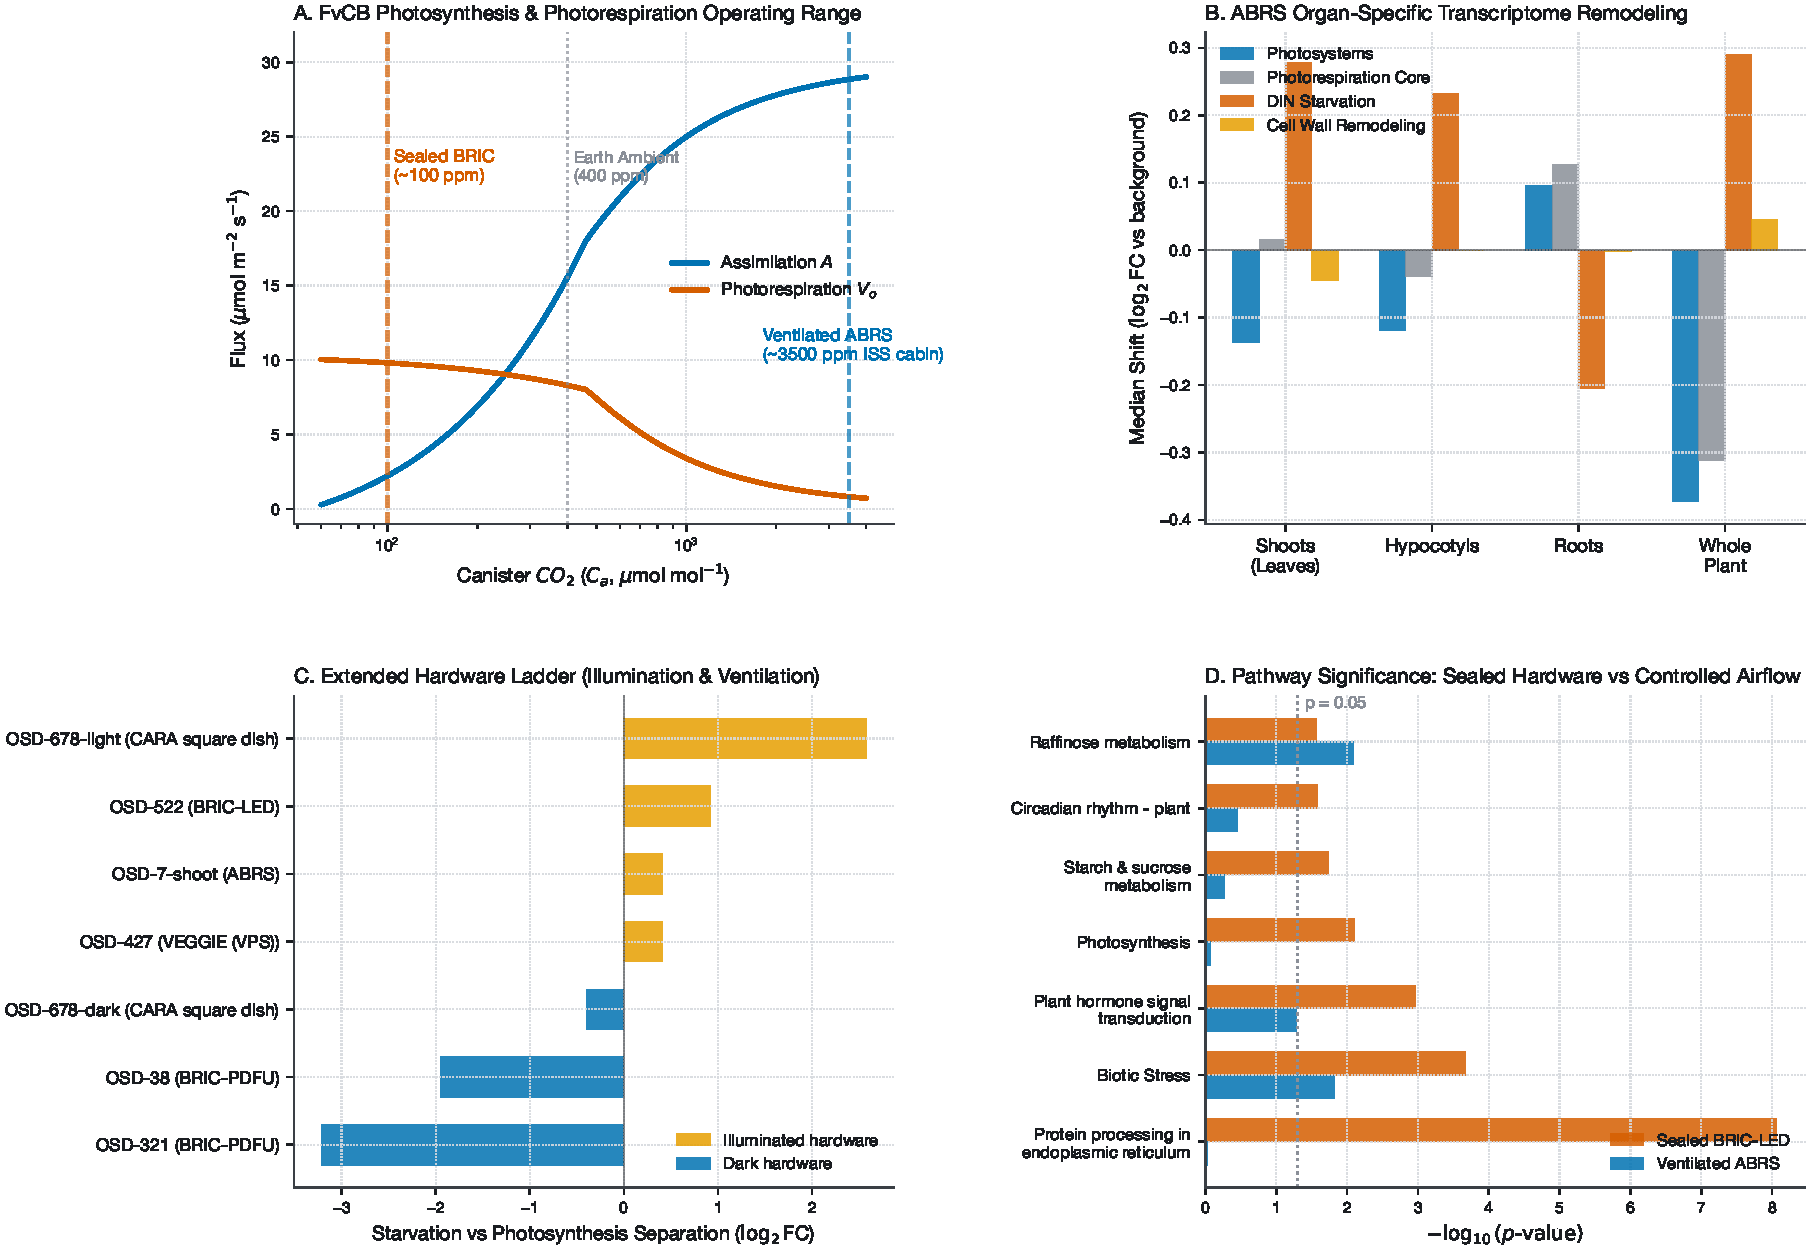
\includegraphics[width=0.95\textwidth]{fig09_abrs_comparison.pdf}
\caption{Ventilated ABRS hardware resolves hardware confounds and validates the extended ladder. \textbf{a}, FvCB operating curves spanning drawn-down canisters (100\,ppm) to super-ambient ISS cabin air (3{,}500\,ppm). \textbf{b}, Organ-specific transcriptome shifts in ABRS across shoots, hypocotyls, roots, and whole plants. \textbf{c}, Extended seven-study hardware ladder demonstrating that illuminated VEGGIE ($+0.4142$) and ABRS ($+0.4146$) converge on an identical unconfounded baseline. \textbf{d}, Pathway significance contrast between sealed BRIC-LED and ventilated ABRS, showing complete disappearance of ER stress ($p = 0.946$) under active airflow.}
\label{fig:abrs}\end{figure}

\clearpage
\bibliography{references}

\end{document}
